%%% Druhá kapitola

\chapter{Robotický Swarm}
V češtině se také používá výraz Rojová Robotika nebo Robotický Roj, v angličtině je známý pod pojmem Swarm Robotics. Myšlenka Robotického Swarmu pochází podobně jako u Genetických Algoritmů z inspirace matkou Přírodou. Podle souhrnu \citep{swarmRobotic} popíši základní myšlenku RS.
\section{Základní vlastnosti}
Motivací pro použití RS může být chování živočichů na Zemi. Zaměříme se na skupiny živočichů jako jsou mravenci, včely, ryby dokonce i některé savce. Pokud bychom vložili do prostředí jednotlivce z některé ze zmíněných skupin, nebude schopen konkurovat nepřátelskému prostředí a nejspíše příliš dlouho nepřežije. Na druhou stranu, když budeme uvažovat celé společenství, tak se nám ze slabého jedince stane velmi adaptivní, odolný a rychle se vyvíjející roj. Podobnému účinku bychom se chtěli přiblížit v RS. Pro relativně jednoduchého robota, který není schopen plnit obtížný úkol, se pokusíme použít vícero robotů stejného typu, kteří společně zadaný úkol vyřeší. Navíc chceme těžit ze všech výhod hejna. \par
Jako nejčastější výhody RS oproti jednomu robotovi se nejčastěji uvádějí:
    \begin{enumerate}
        \item Paralelita - Díky malé ceně jedince, si můžeme dovolit velkou populaci jedinců. Malou cenou jedince v ES myslíme, že se jedná o jednoduchého robota s nízkou pořizovací cenou. V kontextu živočichů můžeme uvažovat množství energie, jídla pro tvorbu takového jedince. Velká populace nám umožňuje řešit vícero úkolů naráz, také na velké ploše. Zvláště pro vyhledávací úkoly ušetříme nemalé množství času. 
        \item Škálovnatelnost - Změna velikosti populace hejna neovlivní chování ostatních jedinců. Samozřejmě plnění úkolu bude rychlejší či pomalejší, ale původní hejno bude stále plnit původní úkol. Tím pádem můžeme celkem snadno upravovat velikost populace bez větší obtíží. V přírodě můžeme pozorovat, že smrt  jednotlivých mravenců-dělníků znatelně neovlivní práci celého mraveniště. Nově narození mravenci se mohou vydat do práce, zatímco zbytek mraveniště nemění činnost. 
        \item Houževnatost - Související se škálovatelností, jen v tomto případě máme na mysli necílenou změnu populace. Jako v předchozím příkladu, u smrti mravenců, část robotů ES může selhat z rozličných důvodů, zbytek hejna však bude pokračovat k cíli, i když ve výsledku jim bude jeho dosáhnutí trvat o něco déle. Což se nám může vyplatit v nebezpečných prostředích. 
        \item Ekonomické výhody - Cena návrhu a konstrukce jednoduchých hejn robotů vyjde většinou levněji než jeden specializovaný robot schopný uspokojit stejné požadavky. V dnešním světě vychází výroba ve velkém množství mnohem levněji než tvorba jednoho drahého konkrétního robota.
        \item Úspora energie - Díky menší velikosti a složitosti jednotlivých robotů vyžadují mnohem menší množství energie. Což má za důsledek, že si u nich můžeme dovolit energetickou rezervu na delší čas. Navíc když je pořizovací cena jednoho robota menší než náklady na dobití, můžeme díky škálovatelnosti pouze připojit nové roboty, což u drahého robota jde málokdy. 
        \item Autonomie a Decentralizace - V kontextu RS musí každý jedinec hejna jednat autonomně, jedinci nejsou řízeny žádnou autoritou. Takže umí pracuje i při ztrátě komunikace. Opět se vychází z chování živých organismů. Pokud se chovají jedinci hejna dostatečně kooperativně, mohou pracovat bez centrálního řízení, důsledkem toho se stává celé hejno ještě flexibilnější a odolnější, hlavně v prostředích s omezenou komunikací. Navíc hejno mnohem rychleji reaguje na změny. 
    \end{enumerate}
\par 
Mimo RS existuje i řada jiných přístupů, které se inspirovaly životem hejn v přírodě. Občas jsou zaměňovány za RS, nejčastěji se jedná o multi-agentní systémy a senzorové sítě (sensor networks). V následující tabulce jsou popsány jejich nejklíčovější vlastnosti. \par
\begin{center}
    \begin{table}[h] \resizebox{\textwidth}{!}{%
    \begin{tabular}{l l l l l @{\hspace{1.5cm}}D{.}{,}{3.2}D{.}{,}{1.2}D{.}{,}{2.3}}
            \toprule
             & \textbf{Robotická hejna} & \textbf{Multi-robotické systémy} & \textbf{Senzorové sítě} & \textbf{Multi-agentní systémy} \\
            \textbf{Velikost populace }& Variabilní ve velkém rozsahu & Malá & Fixní & V malém rozsahu \\
            \textbf{Řízení} & decentralizované a autonomní & centralizované & centralizované & centralizované \\
            \textbf{Odlišnosti} & většinou homogenní & většinou heterogenní & homogenní & homogenní nebo heterogenní \\
            \textbf{Flexibilita} & vysoká & nízká & nízká & střední \\
            \textbf{Škálovnatelnost} & vysoká & nízká & střední & střední \\
            \textbf{Prostředí} & neznámé & známé nebo neznámé & známé & známé\\
            \textbf{Pohyblivost} & ano & ano & ne & vyjímečně\\
            \hline 
    \end{tabular}}
	\caption{Porovnání systémů s více agenty}
    \end{table}
    \end{center}
    Také se liší svojí aplikací Robotická hejna se nejčastěji používají ve vojenských, nebezpečných úkolech a také pro řešení ekologických katastrof. Multi-robotické systémy potkáváme v transportních, skenovacích úkolech, dále pro řízení robotických fotbalových hráčů. Oproti tomu nejčetnější využití senzorových sítí zasahuje do medicínské oblasti, ochrany životního prostředí. Multi-agentní systémy zase nejvíce zasahují do řízení síťových zdrojů a distribuovaného řízení. 
\section{Použití}
Existuje několik vědeckých prací, které studují a navrhují použití RS v reálném nasazení. 
\par 
Některé jsem zmínil už v úvodu této práce, jako například hasičům asistující roboty \citep{fireRobots}.  Kde si robotické hejno klade za cíl usnadnit a podpořit navigaci lidem v nebezpečném prostředí. Jejich využití je ilustrováno záchranou misí ve velkém skladišti. Hasiči mají díky kouři velmi omezenou viditelnost. Tím pádem se lokalizace přeživších, epicenter požárů a další důležitých bodů stává obtížným a zdraví ohrožujícím úkolem. Robotické hejno tedy může prozkoumat celý prostor před vlastním zásahem. Při zásahu ještě asistovat hasičům při orientaci v prostoru. Nezřídka se stává, že zasahující hasič zahyne, protože se v hustém dýmu v objektu ztratil.
\par
Robotická hejna se také ukázala jako užitečná u ekologický pohrom. Španělští vědci testovali jejich použití při úniku ropy \citep{oilSwarm}, či při hledání centra radiace \citep{radiationSwarm}. 
\par 
V prvně zmíněném příkladu autoři mapovali znečištění mořské vody. Dokonce při plavbách bez defektů se do moře uvolňuje palivo, ropa a další nebezpečné látky. Očekává se, že s rostoucí námořní dopravou se rozrostou tyto lokální znečištění ve vážnou hrozbu. Aktuální systémy monitorující znečištění při katastrofách tankerů jsou pro toto využití příliš drahé. Autoři proto navrhují použití hejna dronů, které bude dokumentovat velké vodní plochy a bude schopno odhalovat případné nebezpečí a větší koncentrace cizích látek. Dokonce budou moci na základě získaných informací sledovat znečisťovatele. 
\par
Po jaderné katastrofě se stává explorace zamořené oblasti  v podstatě nemožným úkolem pro lidské průzkumníky. Právě monitorování radiací postiženým územím se stala motivací pro práci \citep{radiationSwarm}. Ve zmiňované práci se autoři soustředí na porovnávání autonomních robotických hejn a RH komunikující s člověkem. V rámci výsledků ukazují, výhody použití robotického hejna pro hledání centra radiace a také že RH interagující s lidmi dosahují lepších výsledků.
\par
Několik prací nezůstalo pouze u simulací a také využívali RS u fyzických robotů. Hlavní motivací pro tuto práci byl fakt, že většinou se řízení RS vytváří  a hlavně testuje pouze v uzavřeném a simulovaném prostředí. Tvůrci se rozhodli pro reálné použití na moři, kde nemohou prostředí jakkoli ovládat či kontrolovat. Snaží se tím ukázat, že i přes šumy a neočekávané situace, RS je stabilní a použitelné pro aplikaci ve skutečném světě. Celé hejno se skládalo z deseti robotů. Jednalo se o malé lodičky s délkou přibližně 60 cm a nízkou pořizovací cenou okolo 300 eur. Každý robot byl  vybaven GPS, WIFI, kompasem. Chování bylo připraveno pomocí evolučních algoritmů v simulaci, konkrétně autoři používají neuroevoluci NEAT, jejich simulace obsahovala 4 podúkoly: navádění, shlukování, rozptylování a monitorování prostředí. Poté bylo stvořené řízení ohodnoceno na vodní ploše. Prezentované výsledky vypadají velmi slibně, chování a úspěšnost řízení se velmi blíží mezi simulací a reálným nasazením. Také potvrzují přítomnost výhodných vlastností ze simulaci v reálném světě, jedná se o robustnost, flexibilitu, škálovatelnost. V neposlední řadě také úspěšnost skládání jednoduchých podúkolů do komplexního chování v rámci hejna, které řeší složitý hlavní cíl.  \citep{aquaticRobots}. 
\section{Řízení robotických swarmů}
Chování swarmů se řadí mezi velmi obtížné úkoly pro svět informatiky. Pro reprezentaci chování se využívá \textit{neuronových sítí}, které se optimalizují pomocí nastavování vah jednotlivých perceptronů, neboť se jedná o velký prostor vstupních informací ze senzorů a prostor pro interakci s prostředím je taktéž velmi rozsáhlý. Přímé prohledávání takto obřího prostoru nepřichází v úvahu, proto v poslední době získávají na oblibě evoluční algoritmy. Mezi nejvíce používané patří evoluční strategie, či genetické programování. \par 

\subsection*{Genetické programování a stromy chování}
V práci \uv{Evolving behaviour trees for Swarm robotics} \citep{Jones2018} se autoři zaměřují na využití genetického programování pro vytvoření chování robotického hejna. Pro řízení hejna navrhují vcelku zajímavé využití stromů chování (SC)(behaviour tree), které mají uplatnění především v herním průmyslu pro akce charakterů, které nejsou ovládány hráčem. Jako optimalizační algoritmus zvolili genetické programování. 
\par
Strom chování je strom, jehož listy interagují s prostředím, vnitřní vrcholy spojují tyto akce dohromady a tvoří rozhodovací a závislostní pravidla. Celý strom je vyhodnocován v pravidelných intervalech, v práci se značí jako \textit{tick}. Opírají se o článek \citep{shoulson2011parameterizing},kde bylo ukázáno, že SC může plnohodnotně reprezentovat konečné automaty, dokonce i když budeme používat pravděpodobností konečné automaty. Jako jedince z hejna zvolili Kilobot, které byl představen Rubensteinen v \citep{Kilobots}. Kilobot se pohybuje pomocí dvou vibračních motorů, komunikují přes infračervený kanál, v prostředí se orientují pomocí foto detektoru a signalizují pomocí LED diod s barevným spektrem. Následující části zjednodušují komunikaci s efektory robota a nad nimi optimalizováno SC. 
\par
\begin{table}[h]\resizebox{\textwidth}{!}{%
		\begin{tabular}{l l l l l @{\hspace{1.5cm}}D{.}{,}{3.2}D{.}{,}{1.2}D{.}{,}{2.3}}
        \toprule
        Efektor/Senzor & Read or Write & Popis \\
        \midrule
        motor & W & vypnut, vřed, vlevo, vpravo \\
        přídavná paměť & R\&W & libovolná hodnota \\
        vysílač signálu & R\&W & vysílá při větší hodnotě než 0.5\\
        přijímač signálu & R & 1 pokud přijímá signál \\
        detektor potravy & R  & 1 pokud světelný snímač vidí potravu\\
        nosič jídla & R & 1 pokud nese jídlo \\
        hustota robotů & R & hustota Kilobotů v blízkosti \\
        $\delta hustota$ & R & změna v hustotě \\
        $\delta vzdálenost_{potrava}$ & R & změna ve vzdálenosti k potravě \\
        $\delta vzdálenost_{hnízdo}$ & R & změna ve vzdálenosti k hnízdu \\ 
        \bottomrule
    \end{tabular}}
	\caption{Parameterizing behavior trees, Motion in Games - podoba stromů}
\end{table}
\par
Tyto akce pak odpovídají listům v SC, vnitřní vrcholy mohou být kompoziční: \textit{seqm}, \textit{selm}, \textit{probm} a tyto mohou mít 2 až 4 syny. Informace procházející mezi vrcholy mohou být následujícího druhu \textit{success}, \textit{failure}, \textit{running}. Zpracovávají informace následujícím způsobem posílají tik do každého syna dokud od nějakého nepřijde hodnota \textit{failure} nebo tik proběhne na všech synech. Pokud proběhne úspěšně tik u všech synů vrací \textit{success}, \textit{failure} jinak. Oproti tomu \textit{selm} vysílá tik, dokud mu nějaký syn nevrátí hodnotu \textit{success} nebo všichni synové provedli tik, pokud se nevrátí jediná hodnota \textit{success}, tak vrací \textit{failure}, v opačném případě \textit{success}. Od obou se liší \textit{probm}, ten s danou pravděpodobností vybere jednoho syna a vrátí jeho odpověď. Vrchol, který má alespoň jednoho syna se statusem \textit{running} vrací stejnou hodnotu. \par
Vrcholy jen s jedním synem patří do jedné z následujících kategorií: \textit{repeat}, \textit{successed}, \textit{failured}. Vrchol \textit{repeat} vrací tik svým synům, s daným počtem pokusů, dokud nedostane hodnotu \textit{success}. Následující dva vrcholy vrací konstantní odpověď na tik dle svého jména, i přesto pošlou tik svému následníkovi. \par
Poslední skupinu vrcholu tvoří tzv. akční vrcholy \textit{ml}, \textit{mr}, \textit{mf}, což ve stejném pořadí jsou: zatoč vlevo, zatoč vpravo, jeď kupředu. Vrcholy pohybu při prvním tiku vrací \textit{running} při druhém \textit{success} K akčním vrcholům také patří \textit{if}, který implementuje porovnávání synů a vrací \textit{success}, pokud porovnání platí. Poslední z akčních vrcholů je \textit{set}, který nastavuje danou hodnotu synům. 
\par
V prostředí jsou s konstantní frekvencí prováděny tzv. \uv{update} cykly. Každý cyklus se skládá ze třech částí po sobě jdoucích částí.  
\par
\begin{enumerate}
    \item Spočítají se hodnoty v synech z vysílaných signálů a prostředí. 
    \item Na SC je proveden tik, což čte a zapisuje hodnoty do synů. 
    \item Pohybové motory jsou aktivovány a vysílání je upraveno, oboje dle zapsaných hodnot do synů.
\end{enumerate}
\par 
Jako zátěžový test používají obvyklý scénář, který spočívá v hledání potravy a jejím odvážení zpět do hnízda. Fitness se hodnotí podle vzdálenosti doneseného jídla, čím blíže k hnízdu tím lépe. Jako optimalizační metodu autoři vybrali genetické programování a používají DEAP knihovnu \citep{deap}. \
Celá populace velikosti $n_{pop}$ je ohodnocena fitness, každý jedinec se hodnotí podle 10 simulací, každá simulace má jinou startovní konfiguraci. Roboti startují vždy na poli o velikosti 5x5, jejich orientace je vybírána náhodně. Běží 300 simulovaných sekund, frekvence update cyklu 8Hz pro vnímání prostředí a u ovladačů s 2Hz. Používané genetické programování implementuje elitimus přenáší $n_{elite}$ nejlepších jedinců do další generace, zatímco zbylá část je zvolena  turnajovou selekcí s velikostí $t_{size}$. Křížící (rekombinační) operátor, který kříží části stromů, je aplikován s pravděpodobností $p_{xover}$ na všechny páry vybrané turnajovou selekcí. Na vzniklé páry se aplikují 3 mutační operátory. \par
\begin{enumerate}
    \item S pravděpodobností $p_{mutu}$ je náhodný vrchol stromu vyměněn za nový náhodně vytvořený 
    \item S pravděpodobností $p_{muts}$ je náhodná větev stromu a je  vyměněna za náhodně zvolený terminál(vyskytující se na této větvi)
    \item S pravděpodobností $p_{mutn}$ je náhodný vrchol vyměněn za nový, ale se stejným počtem argumentů
    \item S pravděpodobností $p_{mute}$ je náhodná konstanta vyměněna za jinou náhodnou hodnotu
\end{enumerate}
Krom simulace 25 nezávislých běhů evoluce. Také byly otestovány algoritmy na reálných strojích, vytrénované chování bylo otestováno 20 běhy s rozdílnou startovací pozicí a ohodnoceni stejnou fitness. 
\par
Výsledky simulace byly více než uspokojivé v simulační části si hejno vedlo o trochu lépe 0.075 z maximální hodnoty 0.12 (minimum 0) a co se týče reálného nasazení vygenerovaného chování 0.058. Což opravdu není velký rozdíl, když přihlédneme k tomu, že evoluce probíhala čistě na simulační rovině.

\subsection*{Genetické algoritmy a neuronová síť}
Cagri a Yalcin používají ve své práci \citep{yalcin2008evolving} práci neuronových sítí místo SC a pro nastavení vah genetického algoritmu. Shodují se s Winfieldem a jeho kolegy, že evoluce mnoho chování robotického hejna přináší zajímavých strategií, která mohou být mnohem komplexnější než explicitně vytvořené chování. Popisují však také obtížnosti použití evoluce, zvláště volbu evolučního algoritmu a efektivnost celého výpočtu. 
\par
Využívají již existujícího simulátoru Cobot2D, pro všechny experimenty bylo použita mapa bez překážek velikosti 400x400. Roboti se pohybují pomocí dvou-kolečkových motorů, orientují se 4 infračervenými senzory a 4 zvukovo-směrovými senzory, v jejich středu je umístěn všesměrový zvukový vysílač. Vysílače mají pevný rozsah kruhu vysílání a dynamickou sílu. Zvukové senzory se rozhodují pouze podle signálů, jejichž vysílače spadají do $90^\circ$ výseče od senzoru a také jejich vzdálenost musí být menší než daná konstanta. Síla signálu se zmenšuje směrem od vysílače a senzory vrací součet sil signálů. Infračervené senzory skenují úsečku dané velikostí a vrací vzdálenost k nejbližšímu průsečíku. V rámci simulace jsou generovány náhodné šumy pro každou interakci s prostředím, aby se simulace přiblížila co nejvíce reálnému nasazení. Pro ovládání robota byla navržena neuronová síť, která má 8 vstupů (4 pro infra-senzory a 4 pro zvukové) a 3 výstupy a není zde žádná skrytá vrstva. Nákres robota a jeho ovládací neuronové sítě můžete vidět na obrázku. \par
\begin{figure}[h]\centering
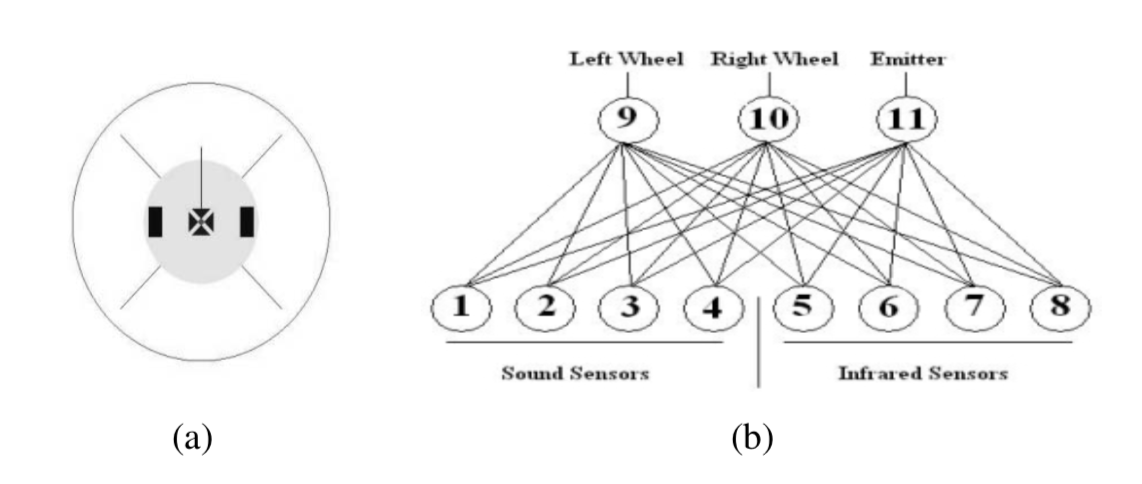
\includegraphics[scale=0.5]{../img/Cobot.png}
\caption{Cobot2D - nákres robota, zdroj : \citep{yalcin2008evolving} }
\end{figure}
\newpage
\textbf{Genetický algoritmus}:
\begin{enumerate}
    \item Inicializuj populaci P 100 jedinců a každý jedinec reprezentován váhovým vektorem
    \item Nastav všem váhovým vektorům z populace náhodné floating point hodnoty v intervalu $\in (-1,1)$ 
    \item $G_{current}$ nastav na 0(id generace)
    \item Dokud $G_{current} < 100$ Prováděj \begin{enumerate}
        \item Pro každý vektor $w \in P$ \begin{enumerate}
            \item Vytvoř 5 simulací prostředí s 10 roboty a orientovanými náhodně
            \item Přiřaď každému roboty jako ovladač neuronovou síť s váhami w
            \item Spust simulaci pro 5000 kroků
            \item Každé simulaci spočítej fitness pro skupinu robotů
            \item Průměr z vypočítaných fitness z předchozího kroku přiřaď jako fitness vektoru w
        \end{enumerate} 
    \item Setřiď vektory podle jejich fitness 
    \item Zvol nejlepších 20 jako elitu $P_{e}$
    \item Zvol náhodně 80 vektorů $P_c$ a aplikuj na ně křížení (prohazuje 1/3 vektoru a shodné páry)
    \item Zvol náhodně 40 vektorů z $P_c$ a aplikuj mutační operátor (přičtení náhodného čísla z $(-1,1)$)
    \item Zvol $P = P_c \cup P_e$
    \item Zvyš $G_{current}$  o jedna. 
    \end{enumerate} 
    \item Vrať jedince, který má z P největší fitness    
\end{enumerate} 
\par 
\textbf{Fitness Funkce}: První použitá $fitness_1$ z tohoto experimentu, obrácená hodnota průměrné vzdálenosti do středu robotické skupiny. 
\par
\begin{center}
\textbf{$fitness_1 = 1/(1/n\sum\limits_{r=1}^{n} d_{rc}) $}
\end{center}
\par 
Kde $n$ je počet robotů v robotické skupině, $r$ je robotův index, $d_{rc}$ je euklidovská vzdálenost mezi $r$ a středem robotické skupiny $c$. 
\par
Druhá $fitness_2$ používá metodu \textit{inverse of hierarchical social entropy} \citep{balch2000hierarchic}. Tato metoda počítá kompaktnost skupiny, tím že hledá každou možnou skupinku (cluster) pomocí změn maximální vzdálenosti $h$ mezi jedinci ze stejného clusteru. Přidávají ještě rozšíření od \textit{Shannon's information entropy}, jenž používá pevné $h$. Toto rozšíření je definováno: 
\par 
\begin{center}
\textbf{$H(h)=-\sum\limits_{k=1}^{M} p_k log_2(p_k)$}
\end{center}
\par 
H se nazývá entropie, $p_k$ je proporce jedince z clusteru $k$, $M$ je počet clusterů pro dané $h$. Konečně celý předpis daný Balchem vypadá následovně: 
\par
\begin{center}
\textbf{$fitness_2 = \int_{0}^{\infty} \frac{1}{H(h)dh}$}
\end{center}
\par 
Použití neuronových sítí a genetického algoritmu se ve výsledku ukázalo jako vhodný prostředek pro učení robotického hejna, neboť se vygenerované chování obstojně shlukuje do úzkých skupin. Definují další tzv. cost funkci pro měření úspěchu nalezených chování, aby mohli porovnávat funkce fitness. A $fitness_2$ se ukazuje jako účinější. 
\subsection*{Evoluční strategie a neuronová síť}
V článku \textit{Self-organised path formation in a swarm of robots} \citep{sperati2011self} aplikují pro řízení robotických hejn evoluční strategie. Jako cíl si článek klade problém průzkumu a navigace v neznámém prostředí v kontextu robotických hejn. Experiment, který měl otestovat uvedené vlastnosti robotického hejna, spočíval v co nejrychlejším přesunu celého hejna mezi dvěma prostory v neznámém prostředí. 
\par 
Pro simulaci bylo využito upravené verze OS Evorobota a jako model jedince z hejna e-puck robot \citep{mondada2009puck}. Tento robot se pohybuje pomocí dvou-koleček, má 8 infračervených senzorů, navíc jeden infračervený senzor na povrch a jeden rozpoznávací barvy vpředu (v tomto případě černobílé prostředí). Navíc mu byla přidělána LED vpředu s modrou barvou a červenou vzadu, která může zapínat a vypínat dle potřeby, a také má snímač barev na vrchu. 
\par
Pro ovládání robota zvolili autoři neuronovou síť se 13 vstupy (8 pro infračervené senzory, 1 pro binární podlahový senzor (bílá vs. černá), 4 pro binární vizuální snímače), dále 3 pro skryté neurony a 4 výstupní neurony (2 ovládající kolečka, 2 aktivující přední a zadní led). Formou jsou podobné předchozím modelům robotů. 
\par
Fitness funkce je vyhodnocena po nasazení do robotů a provedení simulace, vlastní fitness je pak průměr z 15 běhů. Ve vyznačených místech se roboti nabíjí, což trvá daný čas a roboti s lepší efektivitou přesunů z jednoho místa do druhého stihnout cestu tam a zpět mnohem rychleji.
\par 
Výsledky prokazatelně ukazují úspěšné použití evolučních strategií na optimalizaci chování robotického hejna. Pro většinu prostředí dokázali najít efektivní řešení a jak lze vidět na nákresech, dráhy se optimalizují ve dvousměrnou cestu pro přesun z A do B.


